\documentclass[12pt,a4j]{jarticle}
\usepackage{graphicx}
\begin{document}
\title{コンピュータリテラシレポート#13}
\author{2120029 政野玄空}
\date{7月9日}
\maketitle


\section{課題の再掲}
演習2 浦島太郎をもとにしたサイトを作る

\section{レポートの本文}
浦島太郎の物語をベースにしたサイトを作った。それぞれ5つのページとトップページを準備した。
\begin{figure}[htbp]
\begin{center}
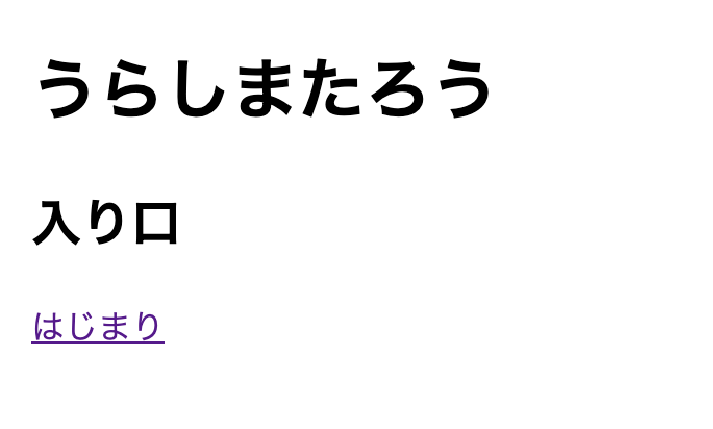
\includegraphics[width=5cm]{taro.eps}
\caption{作成したページの表示です}\label{fig1}
\end{center}
\end{figure}

http://www.edu.cc.uec.ac.jp/\~{}m2120029/top.html

\section{考察}
次へや前へだとわかりにくいのでc課題の目次もあったほうがいいように感じた。
押せないボタンは押せないとわかったほうがいいと思った。
\section{アンケート}

\subsection{Q1:リンクや画像の使用についてどれくらい知っていましたか。}
だいたい知っていた。

\subsection{Q2:CSSによるブロックレイアウトについてはどうでしたか。どのようなページデザインがよいデザインだと思いますか。}
苦手なところだった。見やすくどこを押すとどうなるかひと目で分かるページが良いページだと思う。

\subsection{Q3:リフレクション (今回の課題で分かったこと)・感想・要望をどうぞ。}
CSSが難しかった。

\end{document}
